\documentclass[glossy]{beamer}
\useoutertheme{wuerzburg}
\useinnertheme[realshadow,corners=2pt,padding=2pt]{chamfered}
\usecolortheme{shark}

\usepackage{tikz}
\usepackage{graphics}
\usepackage[utf8]{inputenc}
\newcommand<>{\hover}[1]{\uncover#2{%
    \begin{tikzpicture}[remember picture,overlay]%
        \draw[fill,opacity=0.4] (current page.south west)
        rectangle (current page.north east);
        \node at (current page.center) {#1};
    \end{tikzpicture}}
}

\title{Um framework para geração de testes automatizados para aplicações mobile}
\author{Gustavo Figueira Olegário}
\institute{UFSC}
\date{Florianópolis, 26 de Junho de 2019}

\begin{document}
    \begin{frame}
        \maketitle
    \end{frame}

    \begin{frame}
        \frametitle{Sumário}
        \begin{itemize}
            \item Contextualização e objetivos
            \item Fundamentação teórica
            \item Análise e implementação do framework
            \item Limitações da ferramenta
            \item Resultados obtidos
            \item Trabalhos futuros
        \end{itemize}
    \end{frame}
    \begin{frame}
    \frametitle{Contextualização e objetivos}
        \begin{itemize}
            \item Desenvolvimento de software é caro e demanda tempo de muitas pessoas.
            \item Fases que mais demandam tempo são: desenvolvimento e teste.
            \item Alguns testes produzidos para uma aplicação são triviais de serem
            implementados
            \item Esses testes específicos poderiam ser produzidos de forma automatizada para, então, acelerar o processo.
        \end{itemize}
    \end{frame}
    \begin{frame}
    \frametitle{Contextualização e objetivos}
        \begin{itemize}
            \item Desenvolver uma ferramenta que permita diminuir o tempo investido durante a implementação de testes
            \item Implementar um framework de código aberto que seja capaz de gerar testes automatizados
            \item O framework fica restrito a à aplicações mobile que utilizam  o sistema operacional Android
        \end{itemize}
    \end{frame}
    \begin{frame}
    \frametitle{Fundamentação teórica}
        \begin{itemize}
            \item Frameworks são conjunto de classes que podem ser reutilizados
            em projetos que compartilham o mesmo domínio do problema.
            \item Time de desenvolvimento consegue tirar vantagem do reuso e tem o esforço de implementação reduzido.
            \item Arquitetura já é definida pela ferramenta.
            \item Requer que a equipe saiba utilizar o framework e quais classes
            deve sobrescrever.
        \end{itemize}
    \end{frame}
    \begin{frame}
    \frametitle{Fundamentação teórica}
        \begin{itemize}
            \item Teste de software pode ser definido em diferentes níveis e técnicas.
            \item O mais relevante para esse trabalho: técnica da caixa preta em nível de usuário
            \item Geralmente é o tipo de teste mais difícil de ser escrito e que testa o maior número de funcionalidades do software.
        \end{itemize}
        \begin{figure}
            \centering
            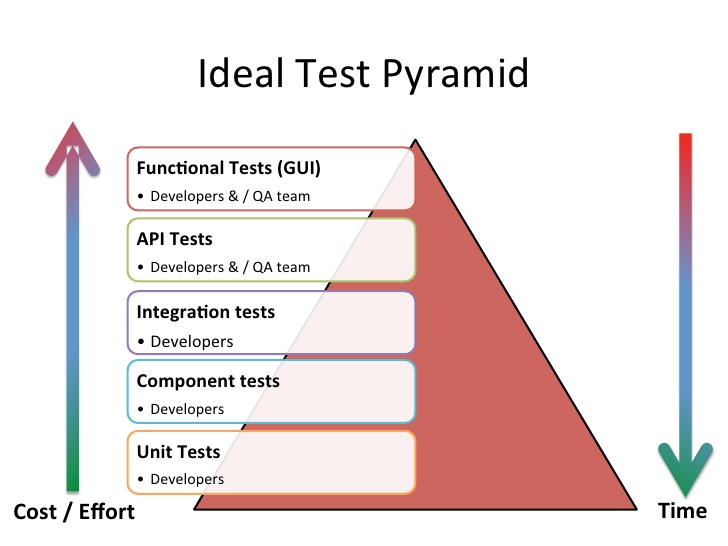
\includegraphics[scale=0.2]{img/pyramid.jpg}
             \caption{\label{fig:passaro}Pirâmide de testes}
        \end{figure}
    \end{frame}
    \begin{frame}
    \frametitle{Análise e desenvolvimento}
        \begin{itemize}
            \item Testes em nível de usuário nada mais são do que ações automatizadas que simulam comportamento de um usuário real.
            \item Teste pode ser escrito automaticamente a partir da captura de ações de um usuário real executando casos de uso de um programa
            \item Framework se responsabiliza em capturar as ações do usuário
            e transformá-las em casos de teste
            \item O teste produzido é exatamente as ações em forma de script
        \end{itemize}
    \end{frame}
    \begin{frame}
    \frametitle{Análise e desenvolvimento}
        \begin{itemize}
            \item Capuccino: framework desenvolvido com o inuito de capturar as interações do usuário com o intuito de produzir os testes em nível de usuário.
            \item Utiliza a API do Android para implementar os métodos que capturam cliques e preenchimento de formulário.
            \item Como complemento utiliza a biblioteca \textit{espresso} para produzir testes em nível de usuário
            \item Mantém as ações do usuário em uma lista ordernada por horário
            em que o evento ocorreu.
        \end{itemize}
    \end{frame}
    \begin{frame}
    \frametitle{Análise e desenvolvimento}
        \begin{itemize}
            \item Usuário deve fazer com que as classes controladoras de GUI herdem de classes específicas do Capuccino.
            \item Usuário deve também herdar uma classe do Capuccino que será responsável por inicilizar a aplicação como um todo.
            \item A asserção para o teste que será produzida fica a cargo do usuário definir.
        \end{itemize}
    \end{frame}
    \begin{frame}
    \frametitle{Análise e desenvolvimento}
        \begin{itemize}
            \item Após configurar o framework usuário deve inicializar a aplicação executando algum caso de uso.
            \item Ao terminar o caso de uso, o usuário deve encerrar a aplicação para indicar ao framework que nenhuma ação será mais executada.
            \item O framework será notificado do término do caso de uso e começará a escrever traduzindo suas estururas de dados internas para a sintaxe do \textit{espresso}.
        \end{itemize}
    \end{frame}
    \begin{frame}
    \frametitle{Análise e desenvolvimento}
        \begin{itemize}
            \item O arquivo produzido pela ferramenta terá um único caso de teste
            \item O teste conterá a asserção definida previamente pelo usuário. Essa asserção deverá também seguir a sintaxe do \textit{espresso}
            \item Com o teste produzido, o usuário pode executá-lo e perceberá que o comportamento automatizado será o mesmo que ele realizou.
        \end{itemize}
    \end{frame}
    \begin{frame}
    \frametitle{Limitações da ferramenta}
        \begin{itemize}
            \item Ações que envolvam operações com rede não são aguardadas até o final quando o teste é produzido.
            \item Eventos de rolagem na tela, apesar de serem suportados pelo framework, não são estáveis devido a inércia do movimento.
            \item A ferramenta só consegue um caso de teste por arquivo. A longo prazo, a base de testes fica grande e ruim de ser gerenciada.
        \end{itemize}
    \end{frame}
    \begin{frame}
    \frametitle{Resultados obtidos}
        \begin{itemize}
            \item Para avaliar a capacidade do framework, implementou-se uma aplicação de compra e venda de produtos
            \item Testou-se a funcionalidade de autenticação da aplicação
            \item Aproximadamente 150 linhas de código produzidas em menos de uma hora.
        \end{itemize}
    \end{frame}
    \begin{frame}
    \frametitle{Trabalhos futuros}
        \begin{itemize}
            \item Implementação de um módulo de rede que permita o framework aguardar operações que envolvam interação com o backend.
            \item Utilizar o framework integrado à um jogo eletrônico e ver como
            ele se comporta.
            \item Implementar um módulo que disponibilize o arquivo de teste direto
            no diretório de testes do projeto.
        \end{itemize}
    \end{frame}
\end{document}
